\documentclass[conference]{IEEEtran}
\IEEEoverridecommandlockouts
% The preceding line is only needed to identify funding in the first footnote. If that is unneeded, please comment it out.
\usepackage{cite}
\usepackage{amsmath,amssymb,amsfonts}
\usepackage{algorithmic}
\usepackage{graphicx}
\usepackage{textcomp}
\usepackage{xcolor}
\def\BibTeX{{\rm B\kern-.05em{\sc i\kern-.025em b}\kern-.08em
    T\kern-.1667em\lower.7ex\hbox{E}\kern-.125emX}}
\begin{document}

\title{DSPtar: Real-Time Guitar Effects on an Embedded Hardware Platform}

\author{\IEEEauthorblockN{Parthiv Krishna}
\IEEEauthorblockA{\textit{Department of Electrical Engineering} \\
\textit{Stanford University}\\
Stanford, CA \\
parthiv@stanford.edu}
}
\maketitle

\begin{abstract}
Effects pedals are a key part of the guitar effects ecosystem; traditionally, effects are implemented using fixed-function analog circuitry. DSPtar is a real-time guitar effects platform implemented on an embedded hardware platform. It is centered around the Teensy 4.0 microcontroller platform and supporting ADC/DAC hardware. Through analog-to-digital sampling, digital processing, and analog-to-digital reconstruction, it can replace several fixed-function analog guitar pedals. We implemented distortion, delay, equalization, and reverb effects on DSPtar to demonstrate the functionality of the platform. We found that the pipeline had acceptable latency and sound quality, though 60 Hz AC mains hum was difficult to avoid. Our results show that, with careful optimizations, embedded platforms can run the multi-stage audio pipelines needed to create convincing guitar effects.
\end{abstract}

\begin{IEEEkeywords}
audio, real-time, embedded, microcontroller
\end{IEEEkeywords}

\section{Introduction}
Guitar effects pedals have augmented the musical range and staying power of the electric guitar since its invention in 1936. Effects like distortion, delay, equalization, and reverb have enabled the guitar to take a central role in bands across vastly varying genres. With carefully selected effects, an electric guitar can be used to create music from jazz and blues to progressive rock and heavy metal. Pedals bring an unmatched versatility to the tone of the electric guitar during both live and recorded performances. Guitarists often use a ``pedal board'' consisting of several chained, analog, fixed-function pedals to create the perfect blend of effects to achieve their desired sound quality. With individual pedals being somewhat expensive, pedal boards can often cost hundreds of dollars to assemble. 

After spending time during the pandemic learning the electric guitar, we were frustrated by the cost of the many pedals needed to recreate the tones in our favorite songs. However, the rise of digital audio production has proven that effects that were traditionally implemented using analog components like resistors, capacitors, and diodes can also be realized using a pipeline of analog-to-digital (ADC) sampling, digital processing, and digital-to-analog (DAC) reconstruction. To explore the potential to implement effects digitally, we developed a low-cost digital audio effects platform (``DSPtar'') that can be used to replace several analog guitar pedals. Since the effects are implemented digitally in software, they can be reconfigured, extended, and improved by writing C++ code. Through the use of the Teensy 4.0, an embedded hardware platform with DSP acceleration, and an audio board with high-quality ADC and DAC circuitry, the DSPtar pedal processes audio in real-time while maintaining the portability of a traditional guitar pedal.

This paper first provides some background on the four primary effects we implemented, then discusses implementation details and considerations for running in a compute-limited and memory-limited environment


\section{Effects Background}

\subsection{Distortion}

Distortion generates a growling tone which is a key part of blues and rock genres, especially hard rock, punk, and metal music. Analog distortion pedals generally use a combination of solid-state transistors, operational amplifiers, and diodes to generate the high gain and nonlinearity needed to create the effect. With sufficiently high gain, the signal may ``clip'' (i.e., reach its maximum possible value) which introduces high-frequency harmonics. A comparison of a pure sine wave and a clipped sine wave is shown in Fig. \ref{fig:dist_fft}; the odd harmonics (i.e. 3x, 5x, 7x, etc. the original frequency) are present in the frequency domain. 

\begin{figure}[htbp]
    \centerline{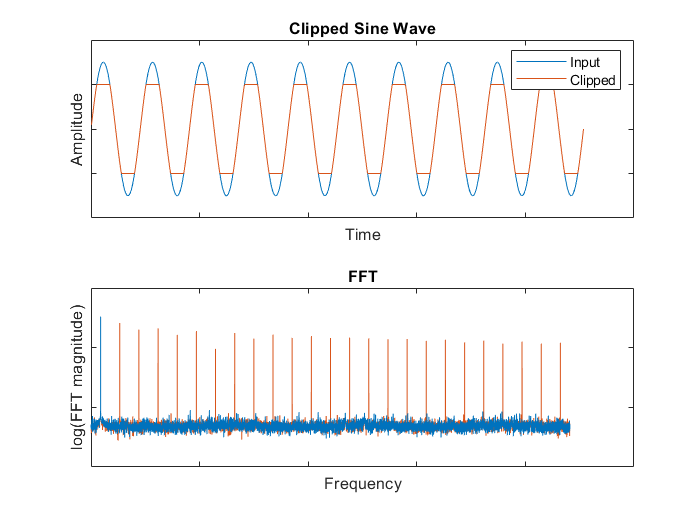
\includegraphics[width=9cm]{dist_fft.png}}
    \caption{Clipped Sine Wave in Time and Freqency Domains}
    \label{fig:dist_fft}
\end{figure}

Digitally, waveshaping can be used to boost the presence of higher frequency harmonics harmonics and change the tone of the sound. Timoney \textit{et al.} \cite{digital_dist} demonstrated that waveshaping can be used to generate distortion effects by introducing more frequency domain content. Waveshaping involves ``mapping'' each level in the input waveform to a different level in the processed output waveform, leading to a different shape of the wave. Several common waveshaping functions are shown in Fig. \ref{fig:waveshape_fns}.

\begin{figure}[htbp]
    \centerline{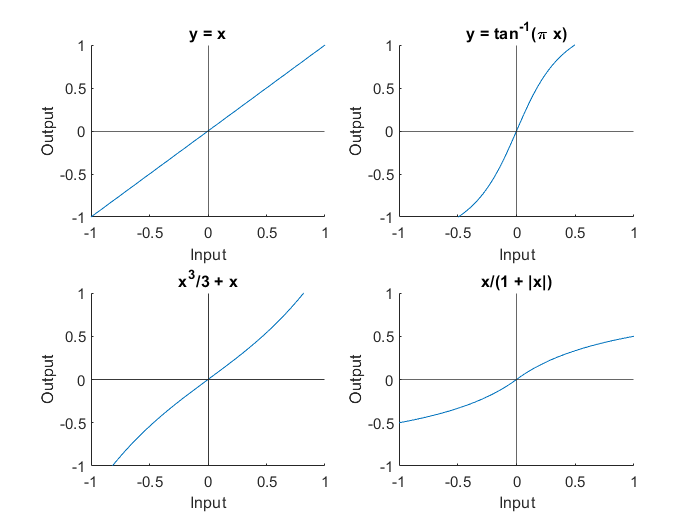
\includegraphics[width=9cm]{waveshape_fns.png}}
    \caption{Waveshaping functions}
    \label{fig:waveshape_fns}
\end{figure}

In each of the examples, an input sample at some level $x$ corresponds to a processed output sample at $y = w_i(x)$. Gain and clipping in tandem with waveshaping can produce a variety of different styles of distortion. 

\subsection{Delay}

Delay is a relatively simple effect that involves combining the input signal with a delayed version of itself. Generally, this can be implemented with a memory that stores input samples. To produce an output sample, the delay effect adds the current input sample to an input sample from $t_{delay}$ seconds in the past. Before adding, the delay effect may also scale the past sample by a factor of $k_{delay}$. Fig. \ref{fig:wilbur_delay} shows the signal from Fig. \ref{fig:wilbur_ir} passed through a delay effect.

\begin{figure}[htbp]
    \centerline{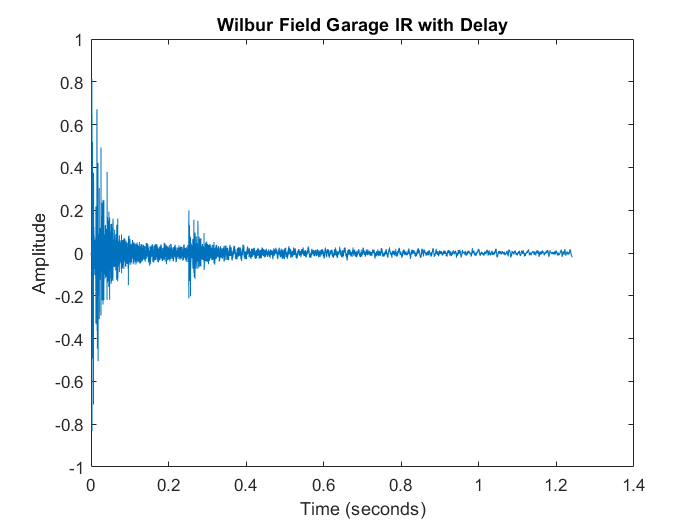
\includegraphics[width=9cm]{wilbur_delay.png}}
    \caption{Impulse response with delay ($t_{delay} = 0.25$, $k_{delay} = 0.25$)}
    \label{fig:wilbur_delay}
\end{figure}

The auditory result is an echo of the input signal. The delay effect may also have multiple delay times $t_{delay,i}$, each with their own scale factor $k_{delay,i}$. Each delay ``tap'' $i$, parametrized by $t_{delay,i}$ and $k_{delay,i}$, contributes an echoed copy of the input signal to the output signal.


\subsection{Equalization}

Equalization changes the relative volumes of different frequencies to change the sonic envelope of an input signal in the frequency domain. EQ can be used to boost certain frequencies of interest (e.g. lower ``bass'' frequencies) or to remove unwanted frequencies (e.g. 60 Hz AC mains hum). It takes the form of a filter, generally envisioned in the frequency domain. A simple of example of equalization is shown in Fig. \ref{fig:eq_sample}; the output is generated by multiplying the input and the EQ curve. This is consistent with the idea of applying a filter in the frequency domain by multiplying the frequency content of the input signal with the frequency response of the filter.

\begin{figure}[htbp]
    \centerline{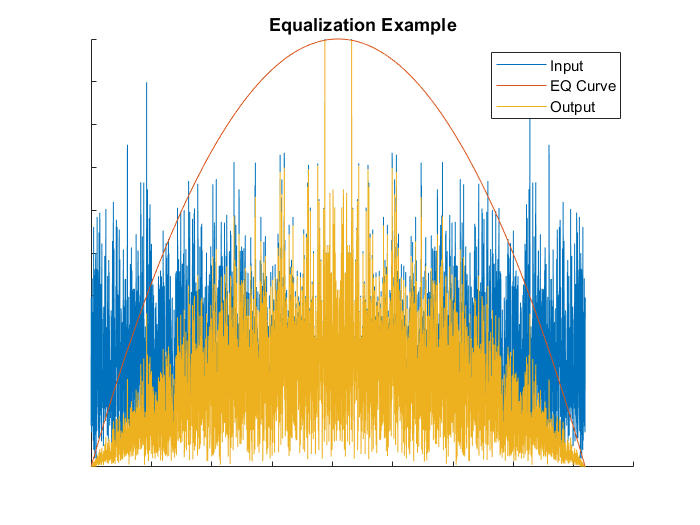
\includegraphics[width=9cm]{eq_sample.png}}
    \caption{Equalization in the frequency domain}
    \label{fig:eq_sample}
\end{figure}

\subsection{Reverb}

At its core, reverb is generated by the reflections of a sound source off of the walls, ceiling, and floor of a space. Common spaces include churches, concert halls, or garages. The space can be modeled as an (ideally) linear system that takes an input ``dry'' signal, applies some linear transform function, and generates an output ``wet'' signal. The response of the space to an impulse, often recorded by clapping, popping a balloon, or generating an electric spark, can be recorded and used to model the space digitally. Then, the reverb effect is generated by convolving the input signal with the impulse response. A sample impulse response of the Stanford Wilbur Field Garage bottom level is shown in Fig. \ref{fig:wilbur_ir}.

\begin{figure}[htbp]
    \centerline{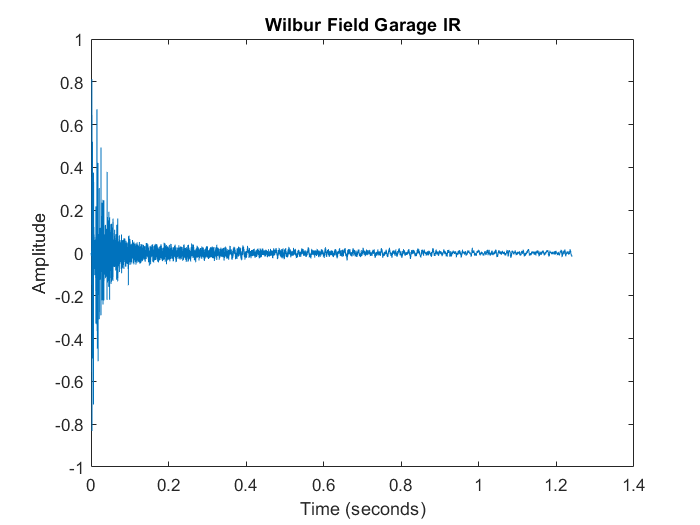
\includegraphics[width=9cm]{wilbur_ir.png}}
    \caption{Impulse response of Wilbur Field Garage LL4}
    \label{fig:wilbur_ir}
\end{figure}

Impulse responses for reverb can also be generated digitally, without recording a ``real-world'' space. In this case, properties like the reverb time, high frequency attenuation, or stereo effects are fully configurable. If recorded and implemented well, the reverb effect provides the illusion that the input sound is being played inside the real or computer-generated space rather than simply being collected through an electronic pickup. This is beneficial in giving the guitar a ``fuller'' tone as it sustains through simulated echoes.



\section{Hardware Platform}

The DSPtar guitar audio effects platform is centered around the Teensy 4.0, a compact microcontroller board with an IMXRT1062 CPU, which implements the ARM Cortex-M7 instruction set. We selected the Teensy 4.0 because its IMXRT1062 chip supports hardware acceleration of vector math and foundational DSP operations like the Fast Fourier Transform (FFT) and Finite Impulse Response (FIR) filtering \cite{arm_dsp_cap}. The acceleration is quite useful when several audio effects need to be processed in real-time.

A Teensy Audio board provides a 44.1 kHz, 16-bit (``CD quality'') ADC and DAC to enable sufficiently high-quality signal conversion from analog to digital and back. The 16-bit audio format is advantageous as it has a relatively high signal-to-noise ratio (SNR) of 96 dB while enabling the software to take advantage of efficient 16-bit math operations. The ARM Cortex-M7 CPU can process 16-bit integers quite efficiently, provided that effects are also implemented with 16-bit integer and/or Q.15 fixed point math operations. The Teensy Audio board reads input using a 1/4" guitar jack that is soldered to the line input of the board; it outputs the processed signals via a pre-attached headphone jack.

\begin{figure}[htbp]
    \centerline{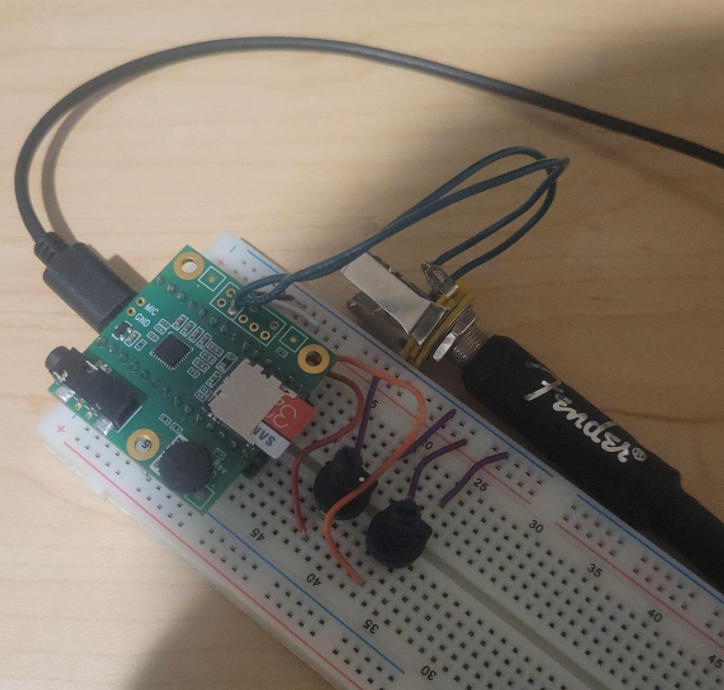
\includegraphics[width=9cm]{dsptar_hw.png}}
    \caption{DSPtar hardware with connected guitar cable}
    \label{fig:dsptar_hw}
\end{figure}


The DSPtar hardware is shown in Fig. \ref{fig:dsptar_hw}. We  soldered the Teensy and Audio board together and placed the assembly on a breadboard to connect two potentiometers for on-the-fly configuration.

\section{Implementation}

The code for DSPtar is available at \cite{dsptar_gh}. The audio pipeline processes effects in blocks of 128 samples to enable real-time operation.

\subsection{Distortion}

We  implemented distortion by writing the \texttt{Preamp} class and the \texttt{Distortion} class in the DSPtar codebase. First, an instance of the  \texttt{Preamp} class receives input samples from the ADC. It applies a gain to the input signal; this gain is configurable using a physical potentiometer enabling the user to change the distortion level in real-time. By multiplying the samples and subsequently hard limiting them at the maximum sample value, the  \texttt{Preamp} generates some harmonic content. 

Second, waveshaping is applied to introduce additional harmonics and reduce the harshness of hard clipping. As described in section II.A, waveshaping applies a transformation function to input samples to generate the associated outputs. However, these transformation functions may be computationally expensive, especially in the case of trigonometric functions or fractional powers. To reduce the overhead associated with computing the waveshaping function of every input sample, the \texttt{Distortion} class uses a precomputed lookup table for waveshaping. We  wrote a MATLAB script that computes the values in Q.15 format and generates a C++ header file that is included in the DSPtar main codebase. 

To save space and avoid storing $2^{16}$ entries for the $2^{16}$ possible int16 values, we  used linear interpolation to compress the lookup table. By selecting a lookup table length $2^n + 1$ for an integer $1 \leq n \leq 15$, we used the following process to find the output value $y$ for a given input value $x$. 

\begin{enumerate}
    \item Add $2^{15} = 32768$ to $x$ to shift it from the $-32768$ to $32767$ range of int16 to the $0$ to $65535$ range of uint16. 
    \item Use the first $n$ bits of $x + 32768$ as the lower index into the lookup table. The value stored here is $y_{lower}$.
    \item Add $1$ to the lower index to get the upper index into the lookup table. The value stored here is $y_{upper}$.
    \item Compute the difference between $d = x \mod 2^{16-n}$; this is the difference between $x$ and the $x_{lower}$ that $y_{lower}$ corresponds to.
    \item Compute the weighted average: $y = \frac{2^{16 - n} - d}{2^{16-n}} y_{lower} + \frac{d}{2^{16-n}} y_{upper}$
\end{enumerate}

This linearly interpolates subsequent lookup table values to efficiently create the waveshaping effect. This code is implemented in the  \texttt{Distortion} class; some bit hacks are used to increase the performance. From the waveshape functions in \ref{fig:waveshape_fns}, we selected the "soft limiting" waveshaper:

$$y = \frac{x}{1 + |x|}$$

The precomputed coefficients are stored in \texttt{distortion\_array.h}.

\subsection{Delay}

Delay can be a challenge to implement in real-time audio systems due to the memory requirements of storing enough samples. Since the input signal must be added after a human-perceptible delay time (hundreds of milliseconds or even seconds), a reverb effect must store a large buffer of samples to be used in the future. At 44.1kHz, storing 2 seconds of int16 samples requires 352.8 kB of space, which is around $\frac{1}{3}$ of the 1 MB of total RAM available on the Teensy. Our implementation of delay uses a ringbuffer to constantly reuse memory and evict old samples.

Each delay tap is confiured with a delay time $t_{delay}$, in ms. Since the data ringbuffer stores audio blocks (\texttt{ringbuffer.h}), the reverb code converts the delay in units of ms to a delay in units of audio blocks $n_{delay}$. When a new audio block is received, the instance of the \texttt{Reverb} class performs the following operations:

\begin{enumerate}
    \item Create an output block and copy the input samples to the output block.
    \item Add the input block to the ringbuffer and evict the oldest block, if necessary.
    \item For each delay tap $i$, peek the $n_{delay,i}$'th most recent audio block in the ringbuffer and multiply it by the delay tap's scale $k_{delay,i}$. For simplicity, this scale is implemented as a right bitshift as delay generally has decereasing amplitude over time.
    \item Add the scaled samples to the output block.
\end{enumerate}

Our initial implementation of this involved copying the input samples into the ringbuffer; this enabled delay times that could be any integer number of samples long. However, the overhead of copying the samples was significant. To circumvent this, the final implementation stores pointers to the existing audio blocks in the ringbuffer. This avoids copying any data, but to simplify the logic, this also restricted delay times to integer numbers of blocks. With each block being approximately $2.9$ ms long, we determined that this was a reasonable constraint given the performance benefits of reducing the enqueue time by two orders of magnitude.

\subsection{Equalization}

Equalization can also be modeled as a linear-time-invariant system. A common feature of equalization effects is the ability to configure the relative volumes of the bass, mid, and treble ranges on the fly, so that the user can tune the tone as desired. This common use case necessitates the ability to be able to modify the filter on-the-fly. Traditional FIR filter design methods like Parks-McClellan would take too long to continually recompute coefficients based on inputs from a physical knob.

We implemented equalization via a cascade of digital biquad filter stages. Flow diagrams for a single filter stage are shown in Figs. \ref{fig:biquad1} and \ref{fig:biquad2}. The filter is parametrized by five filter coefficients, $a_1, a_2, b_0, b_1, b_2$, and has the transfer function

$$H(z) = \frac{Y(z)}{X(z)} = \frac{b_0 + b_1 z^{-1} + b_2 z^{-2}}{1 + a_1 z^{-1} + a_2 z^{-2}}$$.

\begin{figure}[htbp]
    \centerline{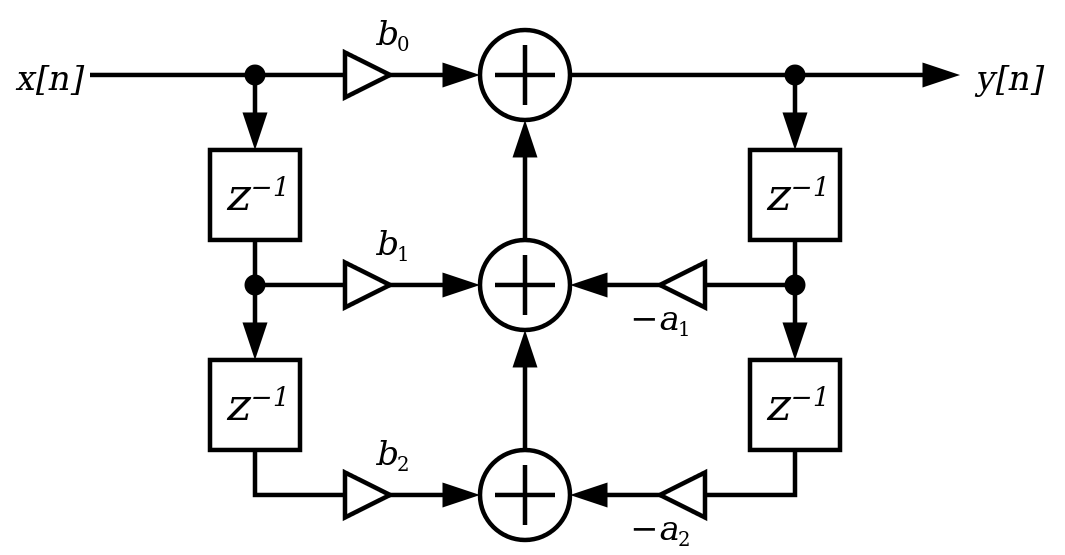
\includegraphics[width=9cm]{biquad1.png}}
    \caption{Flow diagram of a biquad filter, Direct Form 1 (not used) from \cite{biquad_img1}} 
    \label{fig:biquad1}
\end{figure}

\begin{figure}[htbp]
    \centerline{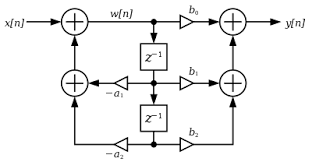
\includegraphics[width=9cm]{biquad2.png}}
    \caption{Flow diagram of a biquad filter, Direct Form 2 (used) from\cite{biquad_img2}}
    \label{fig:biquad2}
\end{figure}

The name ``biquad'' refers to the two quadratic equations that define the transfer function. Though these filters are IIR due to the feedback, they have the benefit of only needing to store a few samples to maintain state compared to a potentially much larger FIR filter state. Between the Direct Form 1 and Direct Form 2 variations, we selected Direct Form 2 (Fig. \ref{fig:biquad2}) because it requires fewer adders, multipliers, and storage than Direct Form 1. The downside of Direct Form 2 is that it increases the possibility of arithmetic overflow, especially for high Q-factors. We reduced the likelihood of overflow by keeping the Q-factors low, generally $\frac{\sqrt{2}}{2}$ or $1$.

Toy \cite{eq_cookbook} describes a set of equations that can be used to generate the biquad filter's coefficients. Given a corner frequency $\omega_0$, define $\alpha$.

$$\alpha = \frac{\sin \omega_0}{2Q}$$


The coefficients for a lowpass filter, with a continuous time frequency response of

$$H(s) = \frac{1}{s^2 + \frac{s}{Q} + 1}$$

are as follows:

$$a_0 = 1 + \alpha$$

$$a_1 = \frac{-2}{a_0}  cos \omega_0$$

$$a_2 = \frac{1}{a_0}(1 - \alpha)$$

$$b_0 = \frac{1}{2a_0} (1 - cos \omega_0)$$

$$b_1 = \frac{1}{a_0} (1 - cos \omega_0)$$

$$b_2 = \frac{1}{2a_0} (1 - cos \omega_0)$$



The coefficients for a highpass filter with a continuous time frequency response of  

$$H(s) = \frac{s^2}{s^2 + \frac{s}{Q} + 1}$$

are as follows:

$$a_0 = 1 + \alpha$$

$$a_1 = \frac{-2}{a_0}  cos \omega_0$$

$$a_2 = \frac{1}{a_0}(1 - \alpha)$$

$$b_0 = \frac{1}{2a_0} (1 + cos \omega_0)$$

$$b_1 = \frac{-1}{a_0} (1 + cos \omega_0)$$

$$b_2 = \frac{1}{2a_0} (1 + cos \omega_0)$$

We also used the provided equations for a 0 dB peak gain bandpass filter, notch filter, lowshelf filter, and highshelf filter from \cite{eq_cookbook}. With these equations, we wrote helper functions for \texttt{EQ} class to set lowpass, highpass, bandpass, notch, lowshelf, and highshelf filters based on the desired cutoff frequencies and Q factors. By setting each stage with different types of filters, the user can generate complex EQ curves on-the-fly and tune them while playing. For example, the value read from a potentiometer could be used to continually feed the \texttt{setLowpass} function, updating the cutoff frequency of the equalization effect.

To implement the filter efficiently, our code uses integer operations with Q.30 coefficients. Thus, the code multiplies 16 bit samples by 32 bit coefficients. We used dedicated multiply-accumulate instructions (i.e. \texttt{smlawt}, signed multiply accumulate word by half-word) to accelerate the process of computing the output value of the filter. These instructions are described in \cite{arm_manual} section A7.7.139. 

\subsection{Reverb}

Reverb is often modeled as a convolution of the original signal with the impulse response of the ``wet'' space (i.e. one with desirable reverberation patterns). If the selected space's impulse response is windowed so that it is finite in length, the reverb takes the form of an FIR filter.

When implementing a reverb, the impulse response is generally human-perceivable in length, on the order of hundreds of milliseconds or seconds. This corresponds to an impulse response length on the order of 10,000 samples, which is significantly larger than the 128-sample blocks in the pipeline. As a result, we elected to use the overlap-and-save method of implementing time-domain convolution in real-time. 

At setup, our code computes the length-256 FFT of overlapping blocks of the provided impulse response. Blocks overlap by 128 samples (the audio block size) and the resulting FFT coefficients are stored in DMA-pinned memory on the Teensy. Storing in DMA memory is beneficial for two reasons. First, the DMA memory provides 512 kB of additional space over the 512 kB main memory that is largely consumed by the delay effect. Second, it allows the FFT coefficients to be readily available to be provided to the DSP coprocessor for complex multiplications. These precomputed FFT coefficients are used repeatedly and don't need to be recalculated.

To compute the output in a given audio block, our code does the following:
\begin{enumerate}
    \item Compute the 256-point real FFT of the audio block concatenated with the previous audio block.
    \item For each block $i$ in the impulse response, perform a complex multiplication with the $i$'th most recent audio block.
    \item Accumulate the various sub-results into a temporary buffer.
    \item Compute the inverse FFT of the temporary buffer to compute the output block.    
    \item Save the current 256-point real FFT to be used on the next iteration.
    \item Save the current samples to be concatenated with the next block on the next iteration.
\end{enumerate}

By using the CMSIS DSP library outlined by Lorenser in \cite{arm_dsp_cap}, we leveraged accelerator and vector hardware on the Teensy to perform the FFT, invese FFT, and complex multiply-accumulates. The result is reverb that runs in real-time with approximately 1 ms of delay, which is even less than the overhead of collecting and outputting one block of 128 samples (2.9 ms * 2 = 5.8 ms).

\subsection{Noise Gate}

Throughout the pipeline, various sources of noise introduce unwelcome artifacts into the audio signal. The most prominent of these is faint 60 Hz AC mains noise that gets amplified in the \texttt{Preamp} and passed further down the pipeline. We used \texttt{EQ} to remove some of this hum; we also wrote a simple \texttt{NoiseGate} effect to remove more of the noise. This effect is configured with a threshold. It outputs the input sample if its absolute value is above that threshold, or zero if the input sample's absolute value is below that threshold. The input-output characteristic of the noise gate is shown in Fig. \ref{fig:noise_gate}.

\begin{figure}[htbp]
    \centerline{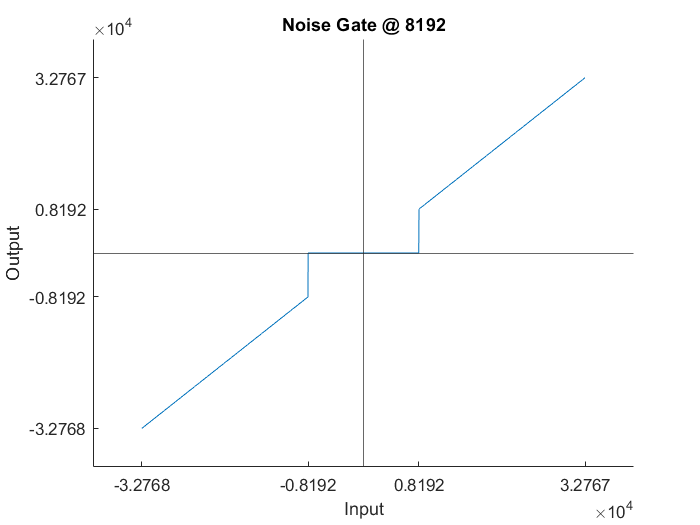
\includegraphics[width=9cm]{noise_gate.png}}
    \caption{Noise gate with threshold = 8192} 
    \label{fig:noise_gate}
\end{figure}

\subsection{Full System}

The overall software pipeline involves processing audio ``blocks'' of 128 samples through each individual effect. The Teensy Audio library \cite{teensy_audio} handles most of the block routing and ensures that audio samples are consumed from the ADC and provided to the DAC. It uses timer-interrupts to ensure that the audio pipeline runs quickly enough to maintain real-time audio processing.

All effects that we wrote inherit from the \texttt{AudioStream} class and define an \texttt{update} function which is called once per block. This \texttt{update} function receives an input block, applies the effect, and transmits an output block. The signals are routed as follows:

\begin{enumerate}
    \item \texttt{AudioInputI2S} collects samples from the audio board's ADC over the I2S protocol.
    \item \texttt{Preamp} applies gain to the signal as described in section IV.A.
    \item \texttt{Distortion} applies waveshaping to the signal as described in section IV.A.
    \item \texttt{Delay} applies delay to the signal as described in section IV.B.
    \item \texttt{NoiseGate} instance removes noise which would be looped through the feedback loops in \texttt{EQ} as described in section IV.E
    \item \texttt{EQ} applies equalization to the signal as described in section IV.C. It sends its output to both the left and right channels of \texttt{Reverb}.
    \item \texttt{Reverb} applies reverb to left and right channels as described in section IV.D.
    \item Two \texttt{NoiseGate} instances (one per channel) remove noise from the signal at the output of reverb before sending to the output.
    \item \texttt{AudioOutputI2S} sends processed samples to the audio board's DAC over the I2S protocol.
\end{enumerate}

We also wrote a main thread that runs outside of the timer-interrupt triggered audio pipeline. It simply reads analog values from the potentiometers and reconfigures the audio effects accordingly. Currently, one potentiometer controls the gain of the \texttt{Preamp} while the other controls the lowpass filter cutoff of the \texttt{EQ}.

\section{Conclusions and Future Work}

Digital audio effects have left their mark on modern sound production for decades, but often rely on bulky computers to process audio signals. Through the DSPtar embedded digital guitar effects platform, the versatility of reprogrammable effects can be had in the size of a traditional fixed-function analog guitar pedal. The low-cost, microcontroller based DSPtar platform can be reprogrammed to emulate any combination of analog guitar pedals, saving the user money and allowing them to experiment with various guitar tones.

From a signal processing standpoint, the DSPtar involved the use of various real-time techniques like block-based processing, filtering in the frequency and time domains, and buffering to store samples. Implementing these on an embedded platform required some careful planning and tradeoffs. However, we found that the Teensy and its ARM Cortex-M7 CPU are quite performant and should be able to support almost any real-time audio processing application. We found that the latency of the overall pipeline was roughly 12 ms; qualitatively, this felt almost immediate when playing the guitar through DSPtar.

Qualitatively, the effects worked well and we found the performance to be satisfactory. Of the effects, \texttt{Distortion}, \texttt{Delay}, and \texttt{Reverb} are the most obvious when listening to the output. We also validated the \texttt{EQ} functionality by sweeping a lowpass filter's cutoff frequency from 10 Hz to 10 kHz. One limitation of the DSPtar is that various sources of noise often added some undesired ``crunchiness'' to the sound. We believe that an isolated power supply, like a 9V battery used in traditional analog guitar pedals, could help reduce the ever-present 60Hz AC mains hum. Though it is possible to cut this frequency with \texttt{EQ}, guitars and bass guitars can produce a 60 Hz note which would be completely removed by the \texttt{EQ}. To reduce noise in a mains-coupled environment, a more sophisticated noise gate (section IV.E) would certainly help reduce the presence of hum and crackles.

In the future, we hope to make the DSPtar easier to use. Some steps we would like to take are 

\begin{enumerate}
    \item Adding more buttons/potentiometers to make it easier to configure DSPtar on-the-fly.
    \item Creating an enclosure to make DSPtar more durable.
    \item Adding a screen to display information about the currently active effects.
\end{enumerate}

Overall, it was challenging but rewarding for us to implement the effects within the compute and memory constraints of the Teensy 4.0 platform. We hope that the insights and ideas in this paper will inspire others to explore DSP applications on embedded hardware.


\begin{thebibliography}{00}
\bibitem{arm_manual} ARM Inc. ``ARM-v7 architecture reference manual,'' ARM DDI, 2014.
\bibitem{biquad_img1} Purple, B. ``Flowchart of a digital biquad filter DF1,'' Wikimedia Commons, July 2021.
\bibitem{biquad_img2} Purple, B. ``Flowchart of a digital biquad filter DF2,'' Wikimedia Commons, July 2021.
\bibitem{dsptar_gh} Krishna, P. ``DSPtar code,'' \\ \texttt{https://github.com/parthiv-krishna/EE264W-DSPtar}.
\bibitem{arm_dsp_cap} Lorenser, T. ``The DSP capabilities of ARM Cortex-M4 and Cortex-M7 processors,'' ARM White Paper, November 2016.
\bibitem{teensy_audio} Stoffregen, P. ``Teensy Audio Library,'' \\ \texttt{https://github.com/PaulStoffregen/Audio}.
\bibitem{digital_dist} Timoney, J., Lazzarini, V., Gibney, A. ``Digital emulation of distortion effects by wave and phase shaping methods,'' Proc. of the 13th Int. Conf. on Digital Audio Effects, September 2010.
\bibitem{eq_cookbook} Toy, R. ``Audio EQ cookbook,'' \\ \texttt{https://www.w3.org/TR/audio-eq-cookbook/}, June 2021.

\end{thebibliography}

\end{document}
